\documentclass{article}

\usepackage{booktabs}
\usepackage{tabularx}
\usepackage{graphicx}
\usepackage{geometry}
\geometry{a4paper, margin=1in}
\usepackage{hyperref}
\usepackage{amssymb}
    \hypersetup{colorlinks=true, linkcolor=blue, citecolor=blue, filecolor=blue,
                urlcolor=blue, unicode=false}
    \urlstyle{same}

% Add the float package for the H specifier
\usepackage{float}

% Increase spacing around figures
\setlength{\intextsep}{12pt plus 2pt minus 2pt}

% Add figure placement control
\renewcommand{\topfraction}{0.9}
\renewcommand{\bottomfraction}{0.9}
\renewcommand{\textfraction}{0.1}
\renewcommand{\floatpagefraction}{0.9}
\setcounter{topnumber}{4}
\setcounter{bottomnumber}{4}
\setcounter{totalnumber}{8}

% Modify section spacing to help with float placement
\makeatletter
\renewcommand \section{\clearpage\@startsection {section}{1}{\z@}%
                                   {-3.5ex \@plus -1ex \@minus -.2ex}%
                                   {2.3ex \@plus.2ex}%
                                   {\normalfont\Large\bfseries}}
\renewcommand \subsection{\@startsection{subsection}{2}{\z@}%
                                     {-3.25ex\@plus -1ex \@minus -.2ex}%
                                     {1.5ex \@plus .2ex}%
                                     {\normalfont\large\bfseries}}
\makeatother

%% Comments

\usepackage{color}

\newif\ifcomments\commentstrue %displays comments
%\newif\ifcomments\commentsfalse %so that comments do not display

\ifcomments
\newcommand{\authornote}[3]{\textcolor{#1}{[#3 ---#2]}}
\newcommand{\todo}[1]{\textcolor{red}{[TODO: #1]}}
\else
\newcommand{\authornote}[3]{}
\newcommand{\todo}[1]{}
\fi

\newcommand{\wss}[1]{\authornote{blue}{SS}{#1}} 
\newcommand{\plt}[1]{\authornote{magenta}{TPLT}{#1}} %For explanation of the template
\newcommand{\an}[1]{\authornote{cyan}{Author}{#1}}

%% Common Parts

\newcommand{\progname}{ProgName} % PUT YOUR PROGRAM NAME HERE
\newcommand{\authname}{Team \#, Team Name
\\ Student 1 name
\\ Student 2 name
\\ Student 3 name
\\ Student 4 name} % AUTHOR NAMES                  

\usepackage{hyperref}
    \hypersetup{colorlinks=true, linkcolor=blue, citecolor=blue, filecolor=blue,
                urlcolor=blue, unicode=false}
    \urlstyle{same}
                                


\title{User Guide\\\progname}

\author{\authname} % Uses the author definition from Common.tex

\date{\today} % Use current date

\begin{document}

\maketitle

\begin{table}[hp]
\caption{Revision History} \label{TblRevisionHistory}
\begin{tabularx}{\textwidth}{p{3cm}p{4cm}X} % Adjusted column widths
\toprule
\textbf{Date} & \textbf{Author(s)} & \textbf{Change}\\
\midrule
\today & Sufyan Motala & Created guide based on final webapp.\\
% Date2 & Name(s) & Description of changes\\ % Example future entry
% ... & ... & ...\\
\bottomrule
\end{tabularx}
\end{table}

\newpage

\tableofcontents

\newpage

% --- Start of User Guide Content ---

\section{Introduction}

\subsection{Purpose of MES-ERP}
The \progname{} (McMaster Engineering Society - Expense Reporting Platform) is a web-based application designed to streamline financial operations for the MES and its associated student groups. It provides a centralized platform for submitting, tracking, and managing reimbursement requests, payment requests, and budgets efficiently and transparently.

\subsection{Purpose of this Guide}
This guide provides instructions on how to effectively use the \progname{} platform based on your assigned role(s). It covers common tasks, navigation, and key features to help you manage your financial activities.

\subsection{User Roles Overview}
The platform uses a Role-Based Access Control (RBAC) system. Your capabilities within the application depend on the role(s) assigned to you. Common roles include:
\begin{itemize}
    \item \textbf{Regular User:} Can submit personal requests and view their status.
    \item \textbf{Club/Group Admin:} Can manage requests, budgets, and potentially users/roles for specific groups they oversee.
    \item \textbf{System Admin (MES Staff/Exec):} Has broad access to manage users, roles, groups, requests, budgets, and system-wide settings.
\end{itemize}

\subsection{User Demo Guide}
For a visual walkthrough of the platform's features and functionality, please refer to our comprehensive video demo guide: \href{https://www.macvideo.ca/media/t/1_ga0b5798}{MES-ERP User Demo Guide}.

\clearpage
\section{Getting Started}

\subsection{Accessing the Platform}
The \progname{} platform is accessible via a web browser on desktops and laptops (Windows, macOS, Linux). It is also accessible on mobile devices (iOS, Android). Ensure you are using a modern browser like Chrome, Firefox, or Edge. The main URL is \href{https://macengsociety.ca/erp}{https://macengsociety.ca/erp}.

\subsection{Logging In}
\begin{enumerate}
    \item Navigate to the login page (typically the application's root URL or \texttt{/login}).
    \item Enter your registered email address and password.
    \item Click the \textbf{Login} button.
    \item Upon successful login, you will be redirected to your dashboard (\texttt{/dashboard/home}).
\end{enumerate}

\begin{figure}[H]
    \centering
    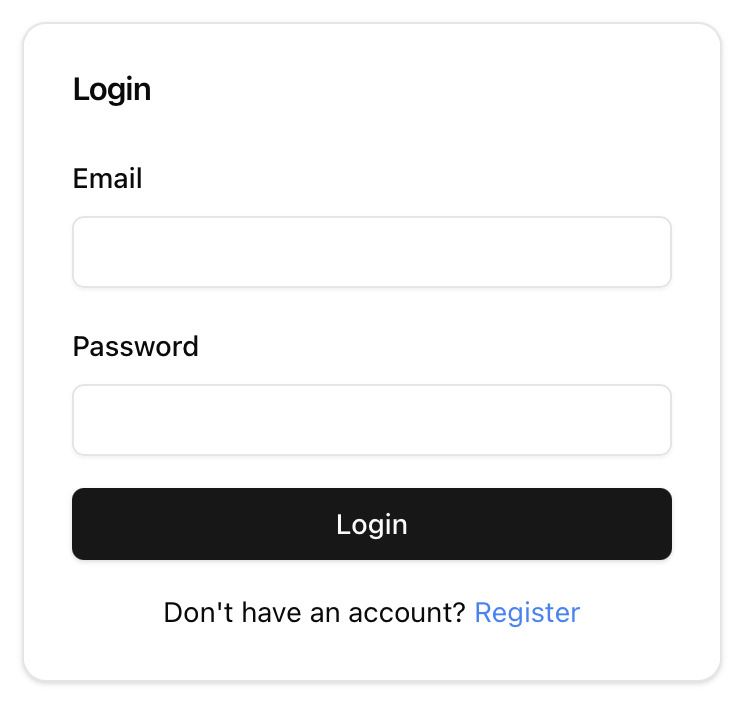
\includegraphics[width=0.8\textwidth]{login_page.png}
    \caption{Login Page}
\end{figure}

\subsection{Registering a New Account}
\begin{enumerate}
    \item From the login page, click the \textbf{Register} link.
    \item Enter your email address and choose a secure password.
    \item Click the \textbf{Register} button.
    \item You may need to check your email to confirm your registration before you can log in.
    \item Upon first login after registration, a user profile will be created for you with a default "user" role.
\end{enumerate}

\begin{figure}[H]
    \centering
    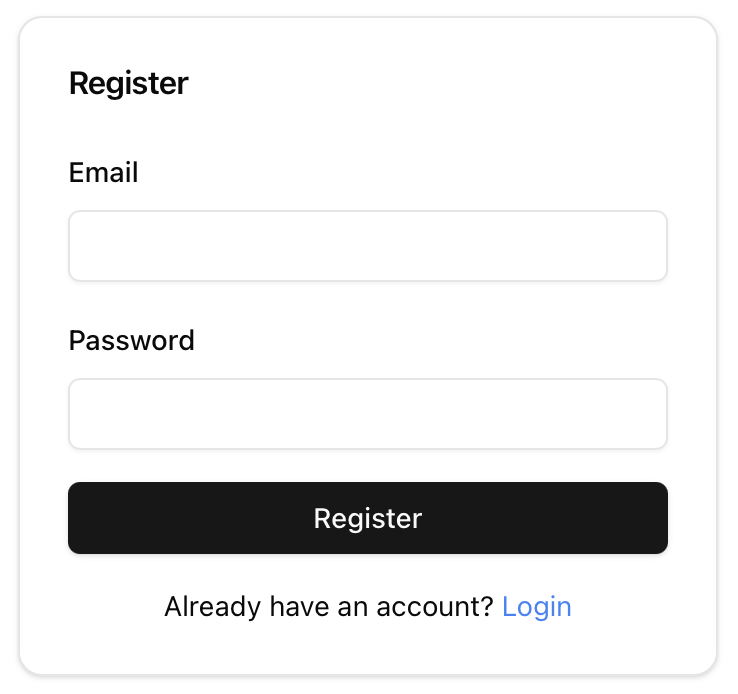
\includegraphics[width=0.8\textwidth]{register_page.png}
    \caption{Registration Page}
\end{figure}

\subsection{Dashboard Overview (\texttt{/dashboard/home})}
This is your main landing page after logging in. It provides a quick overview of relevant statistics based on your role:
\begin{itemize}
    \item \textbf{Regular Users:} See stats for \textit{your} submitted requests (count, total amount).
    \item \textbf{Club Admins:} May see stats for \textit{your club's} requests (total count, amount, pending count) in addition to your personal stats, depending on permissions.
    \item \textbf{System Admins:} See system-wide stats (total requests, total amount, pending count, total users).
\end{itemize}

\begin{figure}[H]
    \centering
    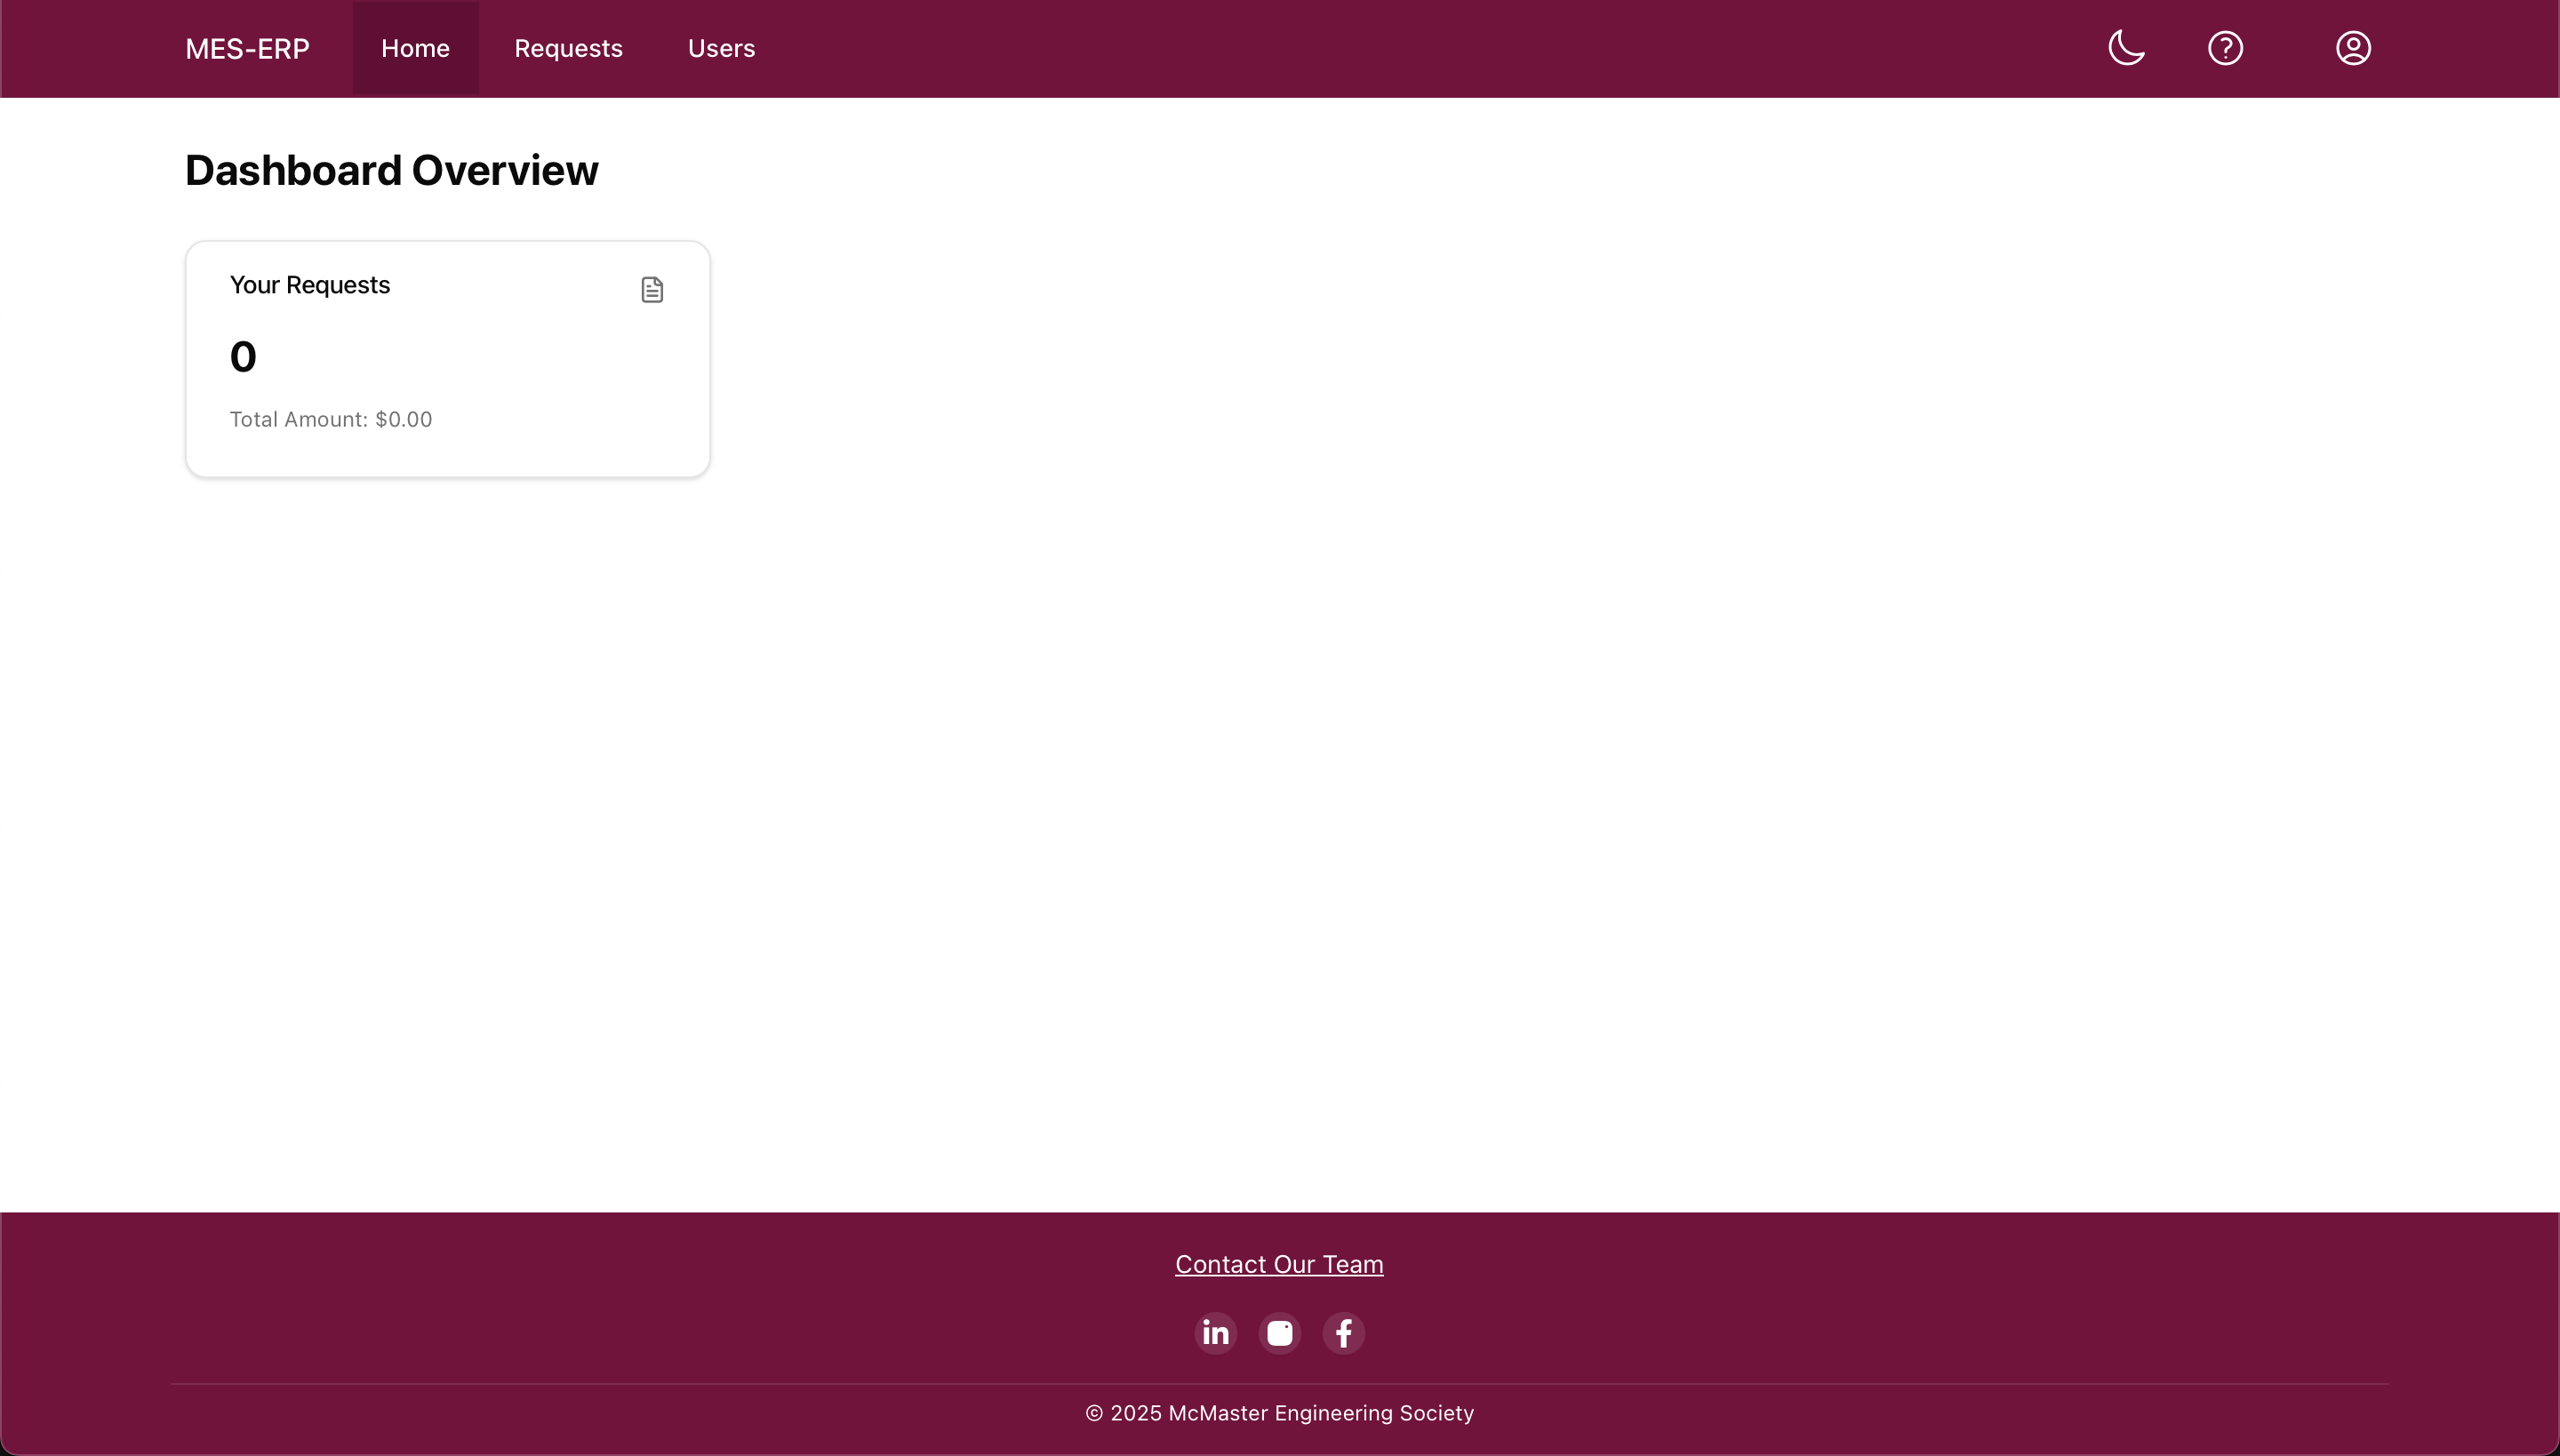
\includegraphics[width=0.8\textwidth]{user_dashboard.png}
    \caption{User Dashboard Home Page}
\end{figure}

\subsection{Navigating the Platform (Header \& Sidebar)}
\begin{itemize}
    \item \textbf{Header:} The header (maroon/dark blue bar at the top) contains the main navigation links (Home, Requests, Users, etc.). The links visible depend on your permissions. It also includes theme toggles, a link to this guide (\texttt{/dashboard/guide}), and the user menu (profile icon).
    \item \textbf{User Menu:} Clicking the profile icon in the header opens a dropdown to access your "Account" page (\texttt{/dashboard/accountInfo}) or "Sign Out".
\end{itemize}

\begin{figure}[H]
    \centering
    
\includegraphics[width=0.8\textwidth]{header.png}
    \caption{Header with Navigation Links and User Menu}
\end{figure}

\subsection{Theme Selection (Light/Dark)}
Click the Sun/Moon icon in the header to toggle between light and dark themes. Your preference is saved locally in your browser.

\clearpage
\section{Guide for Regular Users}

\subsection{Viewing Your Dashboard (\texttt{/dashboard/home})}
See section 2.4 for details. Your dashboard shows stats specific to \textit{your} activity.

\subsection{Submitting Payment/Reimbursement Requests (\texttt{/forms})}
\begin{enumerate}
    \item Navigate to the \textbf{Requests Page} via the header link (\texttt{/dashboard/requests}).
    \item Ensure the \textbf{Payment Requests} tab is selected.
    \item Click the \textbf{Create New Payment Request} button. This redirects you to \texttt{/forms}.
    \item \textbf{Fill out the form:}
        \begin{itemize}
            \item \textbf{Group Selection:} Select the Club/Group this request is for from the dropdown. This is crucial.
            \item \textbf{Basic Info:} Verify or fill in your name, email, phone. Select "Who Are You?" (e.g., MES Position, Club Member).
            \item \textbf{Receipt Upload:} Upload an image (PDF, JPG, PNG) of your receipt OR provide a direct link to the receipt image. The system may attempt OCR to extract the total amount automatically.
            \item \textbf{Role \& Budget:} Select your role and the relevant budget line for this expense.
            \item \textbf{Approval Info:} Enter the name of the individual or project approved for this expense.
            \item \textbf{Team Info (If applicable):} Select sport/team name, conference details if relevant.
            \item \textbf{Payment Details:} Specify if it's a Reimbursement or Payment, the currency, the amount requested (verify if OCR filled it), payment timeframe (date), and preferred payment method (E-Transfer, Direct Deposit, Cheque).
            \item \textbf{Payment Method Details:} Provide necessary details based on your chosen method (e.g., email for E-transfer, bank info for Direct Deposit, address for Cheque).
        \end{itemize}
    \item Review all information carefully.
    \item Click the \textbf{Submit} button. You should see a confirmation message.
\end{enumerate}

\begin{figure}[H]
    \centering
    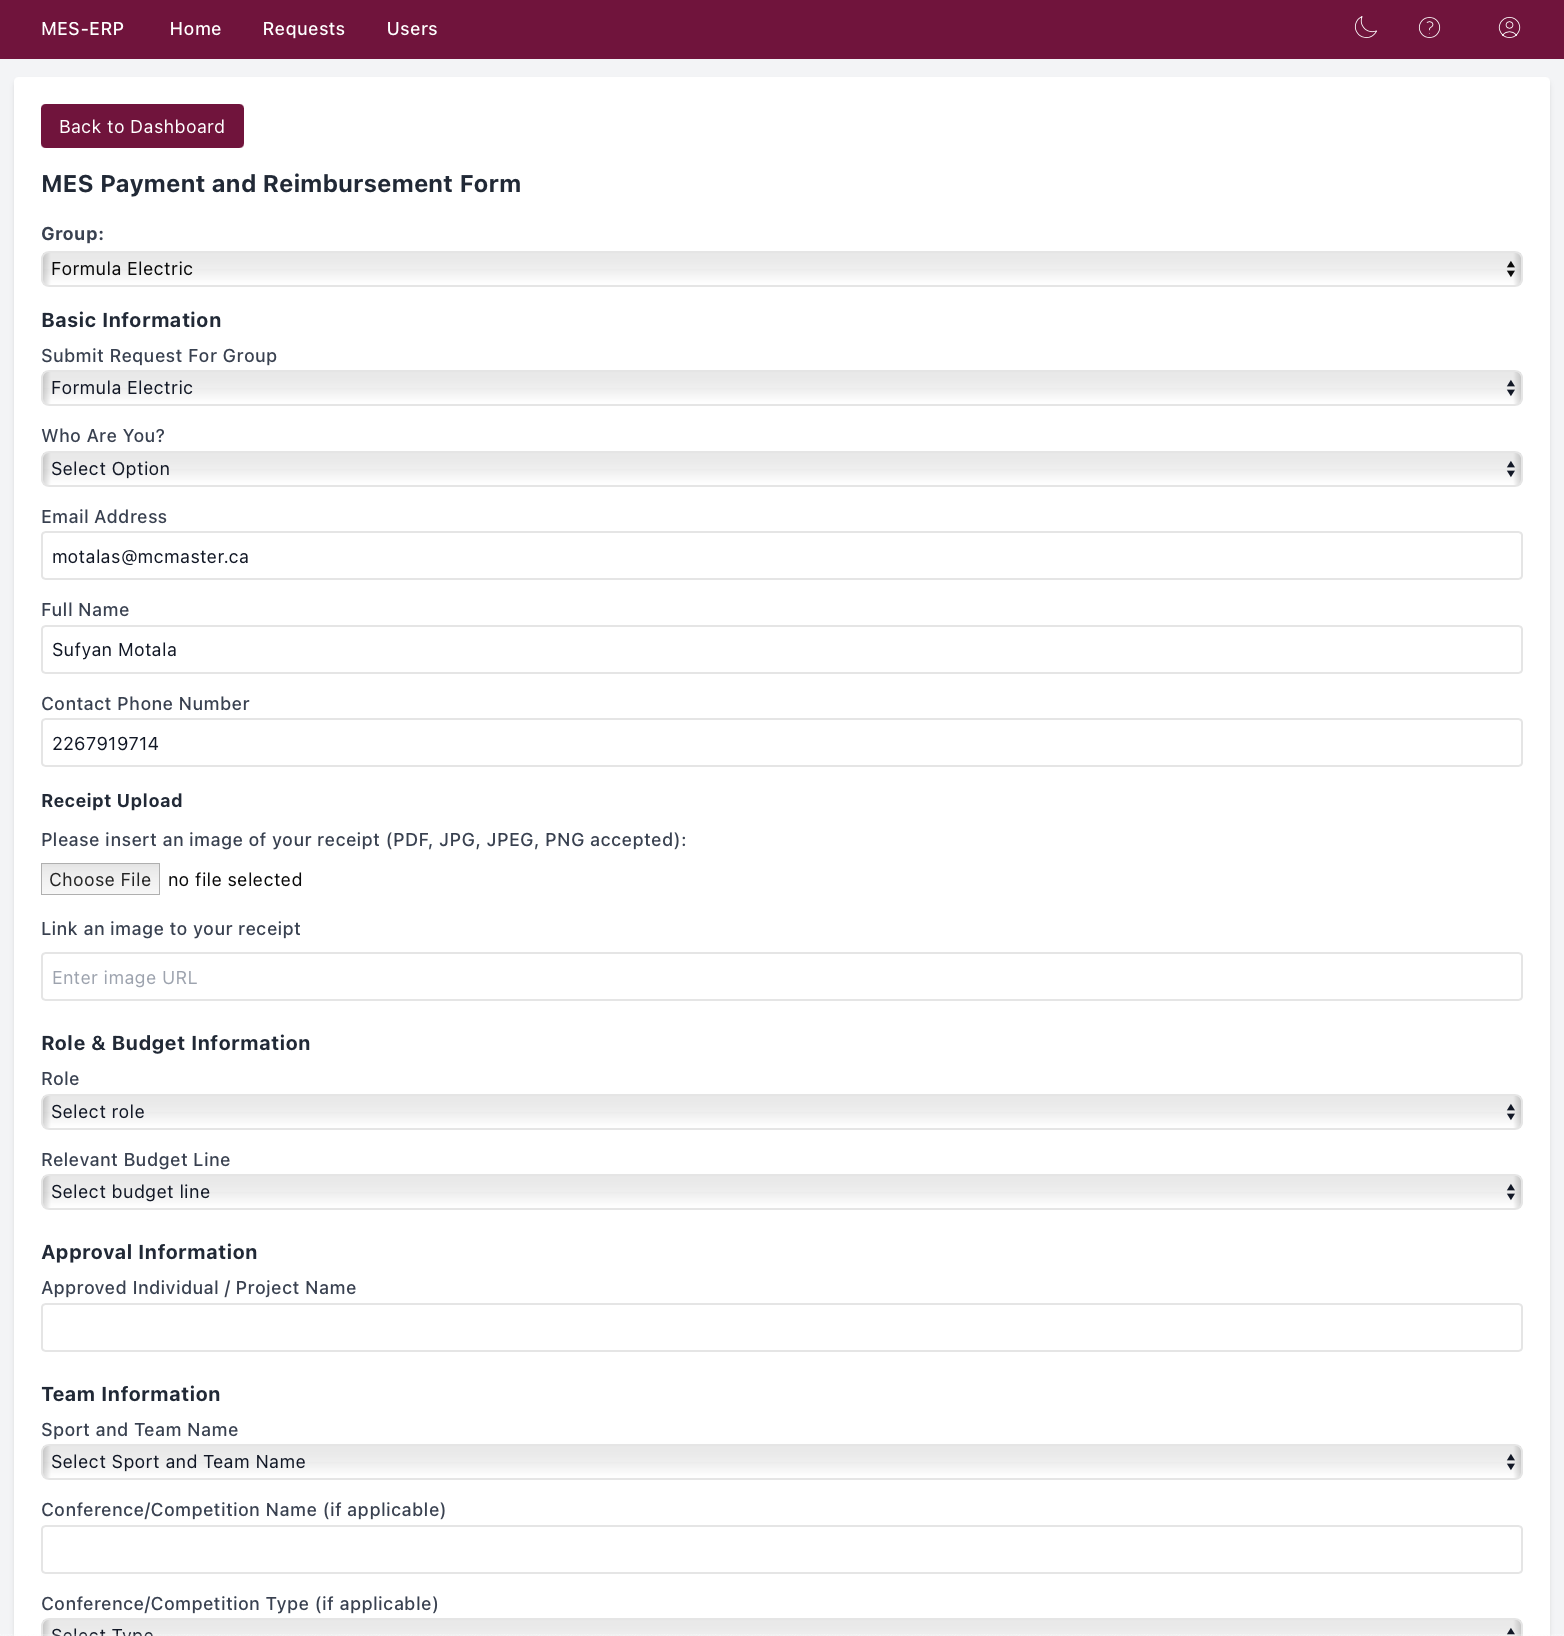
\includegraphics[width=0.8\textwidth]{reimbursement_form.png}
    \caption{Reimbursement Form}
\end{figure}

\subsection{Tracking Your Request Status (\texttt{/dashboard/requests})}
\begin{enumerate}
    \item Navigate to the \textbf{Requests Page}.
    \item The \textbf{Payment Requests} tab will display a table listing \textit{only} the requests you have submitted.
    \item The table shows the request details and the current \texttt{Status} (e.g., Submitted, In Progress, Approved, Rejected, Reimbursed).
    \item You will receive email (and potentially SMS if configured) notifications when the status of your request is updated by an admin.
\end{enumerate}

\begin{figure}[H]
    \centering
    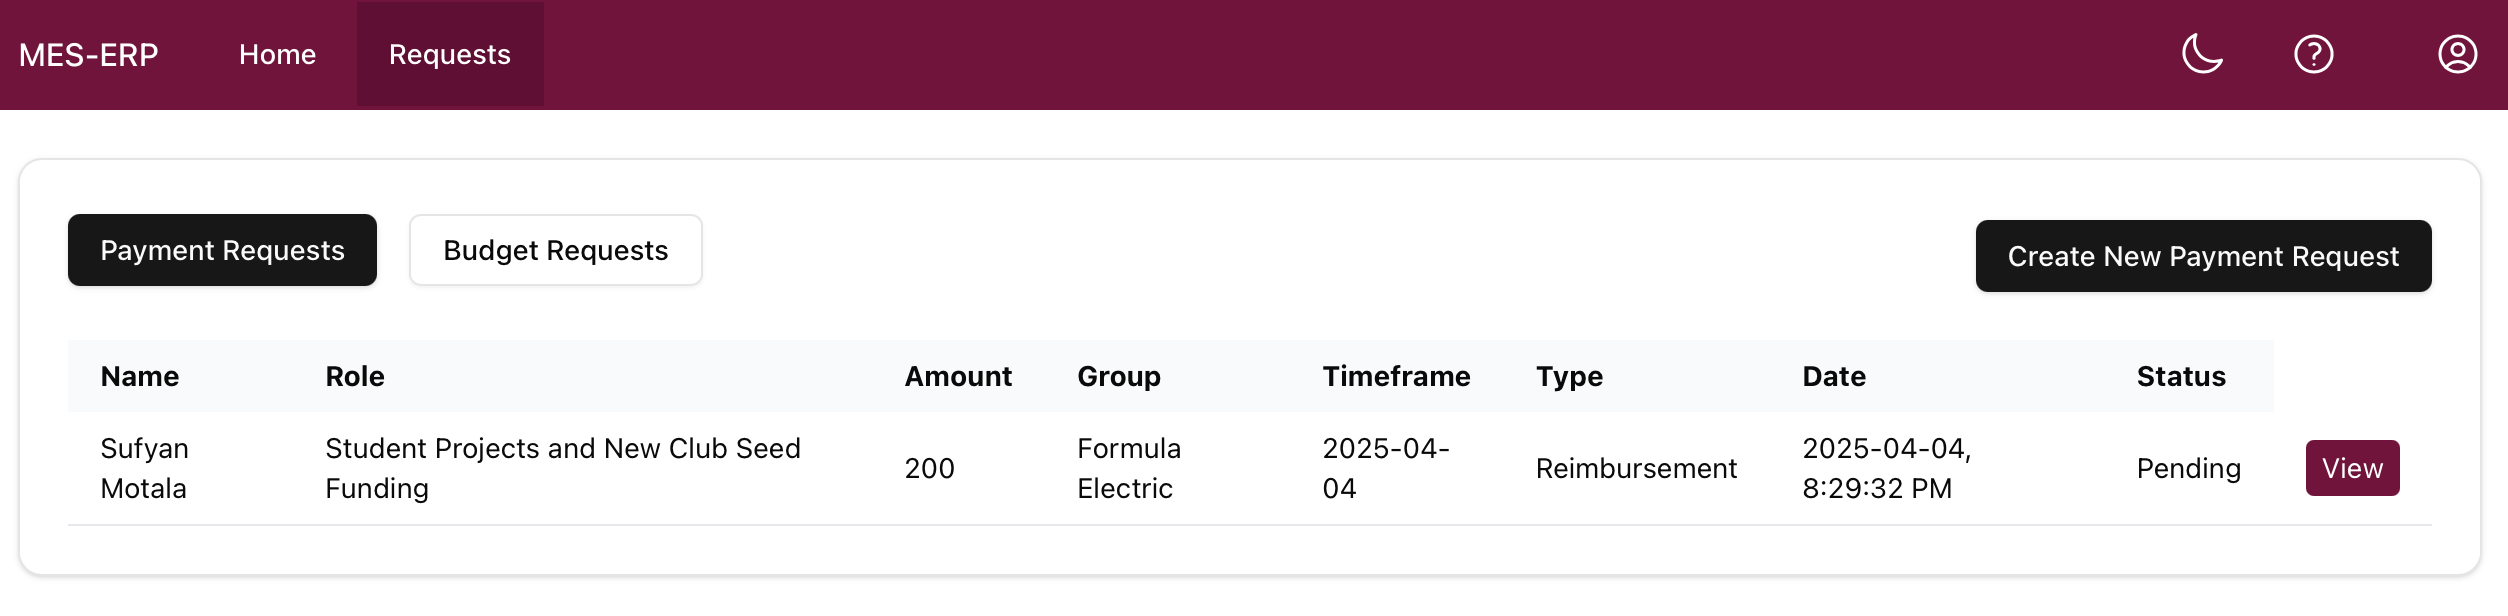
\includegraphics[width=0.8\textwidth]{current_user_requests.png}
    \caption{Requests Page showing User's Requests}
\end{figure}

\subsection{Managing Your Account Information (\texttt{/dashboard/accountInfo})}
\begin{enumerate}
    \item Access this page from the user menu in the header.
    \item View your profile details (email, name, phone number, default payment preference).
    \item Click the pencil icon next to editable fields (like phone number, payment preference) to make changes.
    \item Enter the new value and click the checkmark icon ($\checkmark$) to save, or the X icon (\textsf{X}) to cancel.
    \item \textbf{Note:} Your email address and assigned roles are usually not editable here and must be changed by an administrator.
\end{enumerate}

\begin{figure}[H]
    \centering
    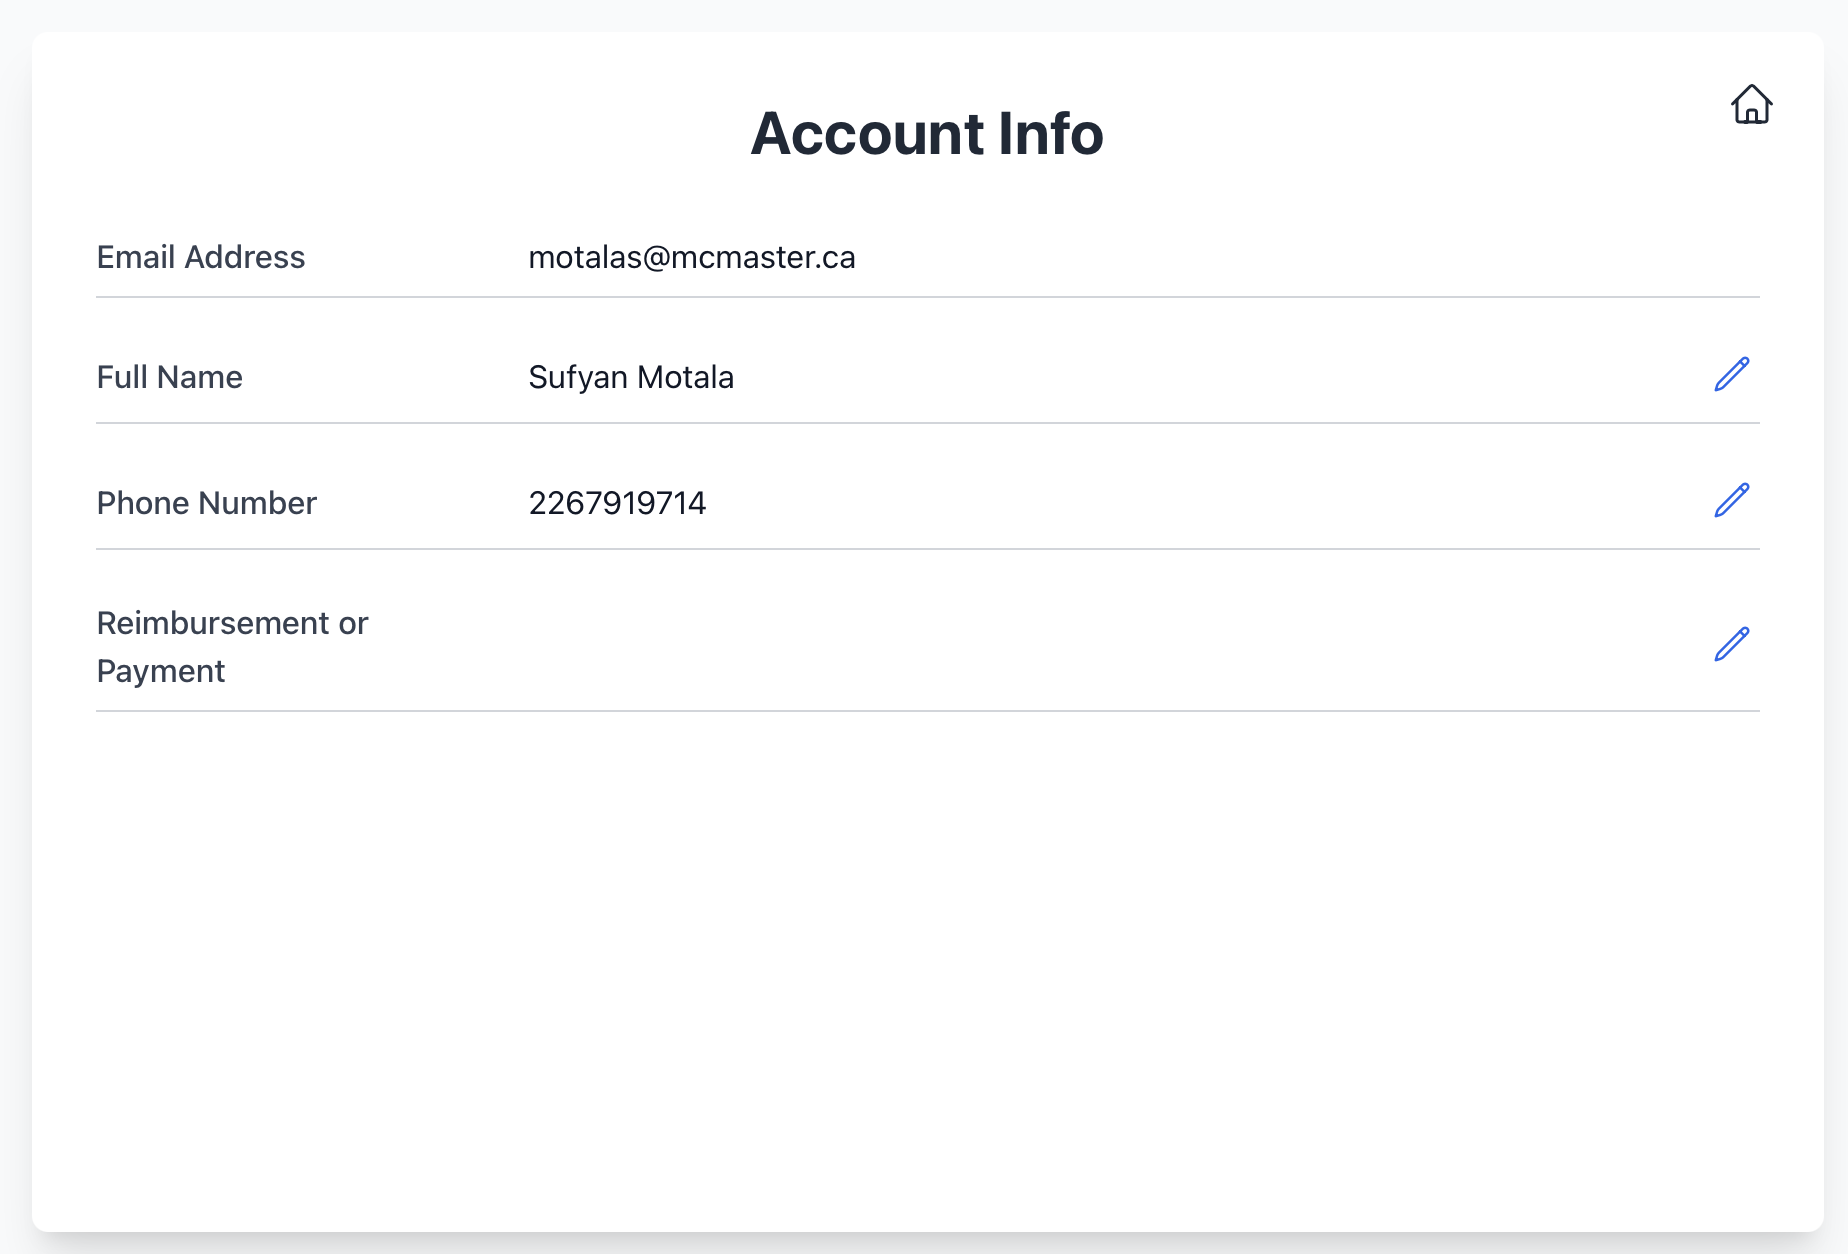
\includegraphics[width=0.8\textwidth]{account_info.png}
    \caption{Account Info Page}
\end{figure}

\clearpage
\section{Guide for Club/Group Admins}
(Requires specific permissions like \texttt{view\_club\_requests}, \texttt{manage\_club\_requests}, etc.)

\subsection{Dashboard Overview (Club-Specific)}
Your dashboard (\texttt{/dashboard/home}) may show aggregated statistics for the specific club(s) you manage, such as total requests, total amount spent, and pending requests within those clubs, in addition to your personal stats.

\subsection{Viewing Club Requests (Payment \& Budget) (\texttt{/dashboard/requests})}
\begin{enumerate}
    \item Navigate to the \textbf{Requests Page}.
    \item The tables here will display requests associated with the group(s) you have permission to view.
    \item Use the tabs (\textbf{Payment Requests}, \textbf{Budget Requests}) to switch between request types for your group(s).
\end{enumerate}

\subsection{Managing Club Requests (Approving/Rejecting)}
(Requires \texttt{manage\_club\_requests} permission)
\begin{enumerate}
    \item On the \textbf{Requests Page}, you will see controls (e.g., a dropdown menu) in the "Status" column for requests belonging to your group(s).
    \item Select a new status (e.g., "Approved", "Rejected") from the dropdown to update the request.
    \item Updating a \textit{payment request} status triggers an email/SMS notification to the submitter.
\end{enumerate}

\subsection{Submitting Payment Requests for Your Club (\texttt{/forms})}
Follow the same process as Regular Users (Section 3.2), ensuring you select the correct Club/Group in the form.

\subsection{Submitting Annual Budget Forms (\texttt{/dashboard/annual\_form})}
(Requires relevant budget permissions)
\begin{enumerate}
    \item Navigate to the \textbf{Annual Budget Form} page (via sidebar or the "Budget Requests" tab on the Requests page).
    \item Fill out the detailed form with projected income and expenses for the specified budget year for your club.
    \item Submit the form for review by MES Finance/Execs.
\end{enumerate}

\begin{figure}[H]
    \centering
    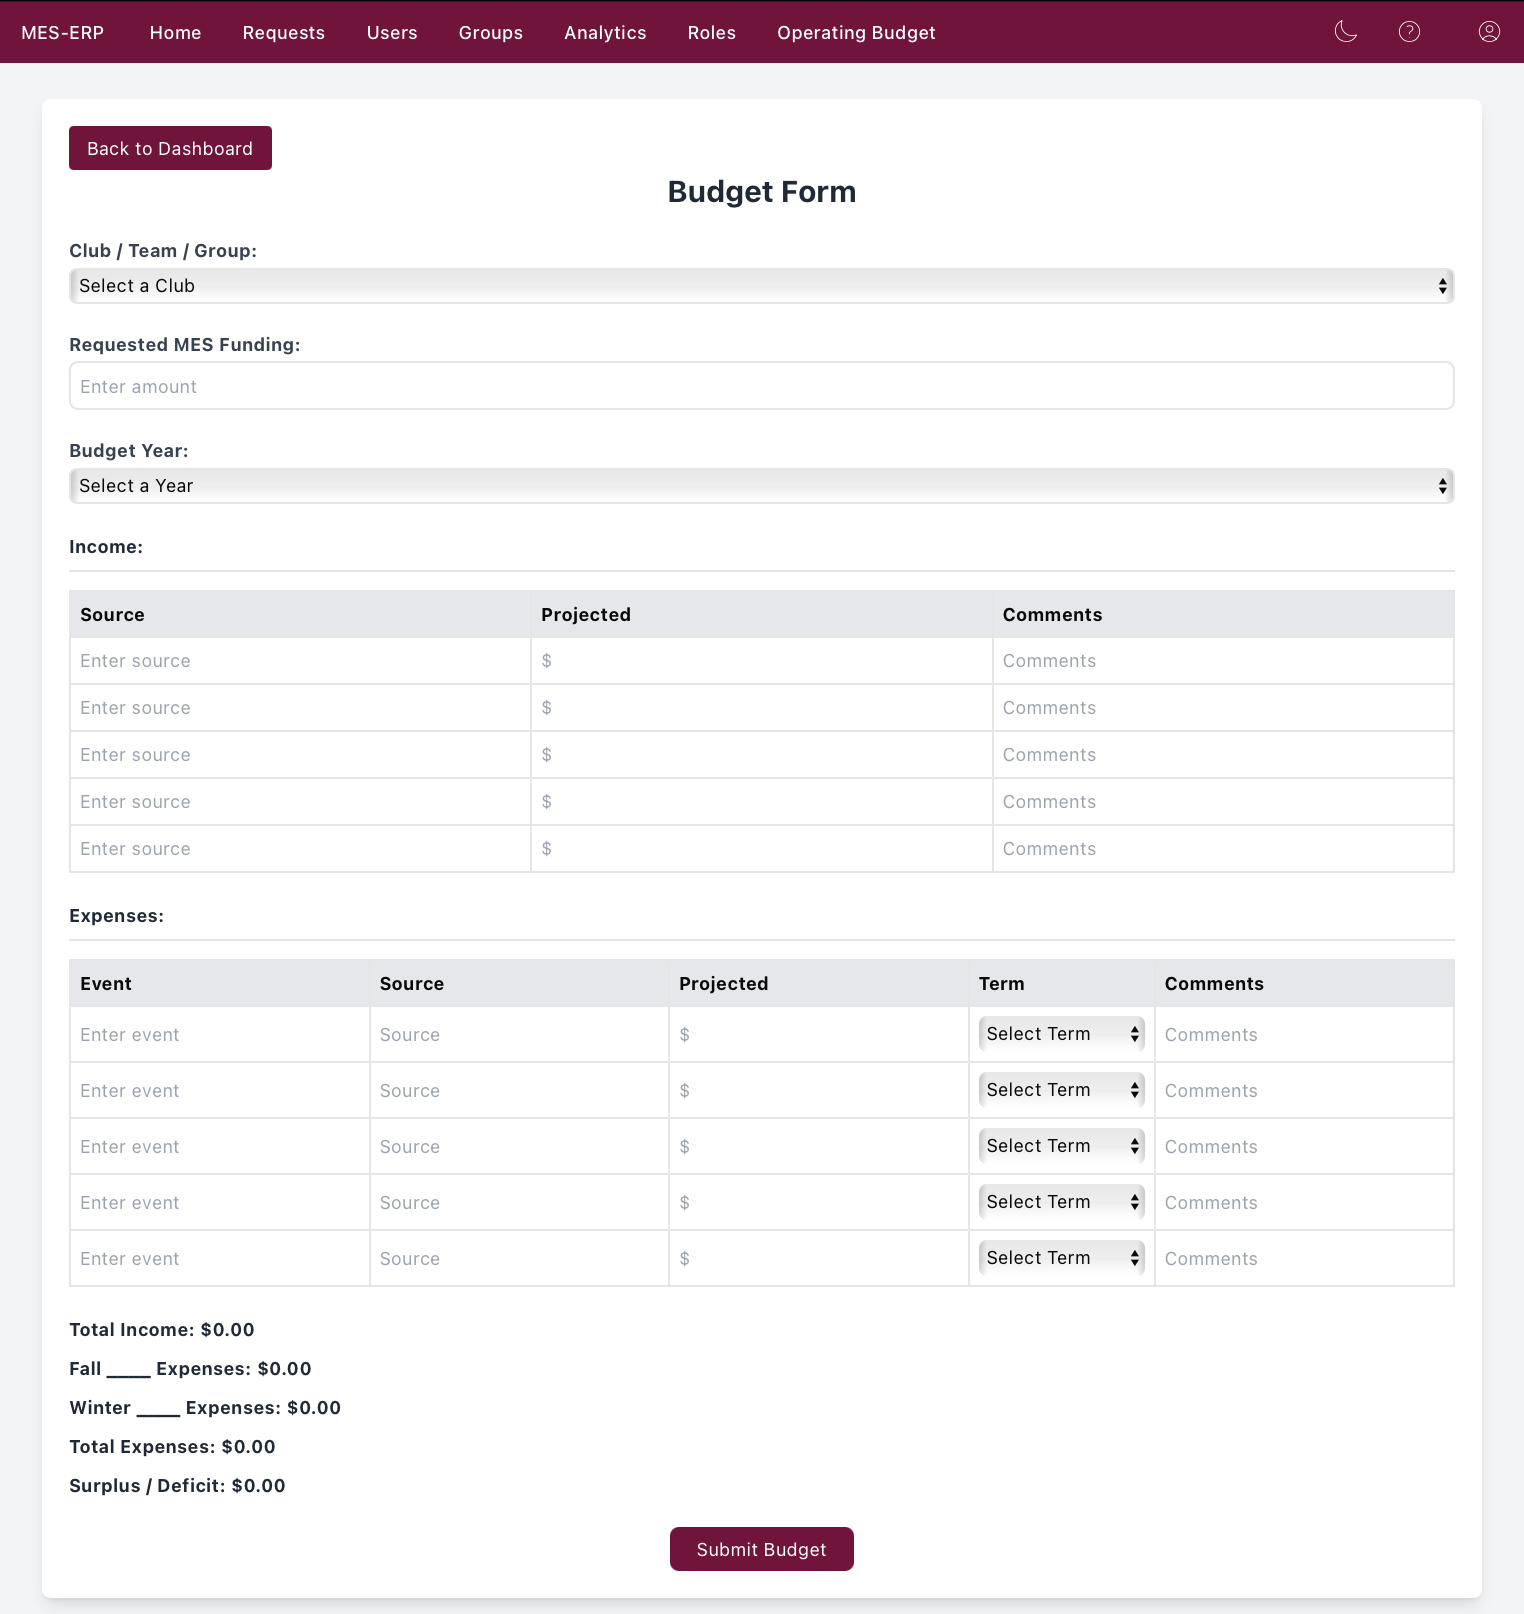
\includegraphics[width=0.8\textwidth]{budget_request.png}
    \caption{Annual Budget Form}
\end{figure}

\subsection{(Optional) Managing Club Members (\texttt{/dashboard/users})}
(Requires \texttt{manage\_club\_users} permission)
\begin{enumerate}
    \item Navigate to the \textbf{Users} page.
    \item You will see a list of users \textit{only within the group(s) you manage}.
    \item You may be able to assign group-specific roles (see below) to these users or potentially remove users \textit{from your group}. You cannot manage users outside your assigned groups.
\end{enumerate}

\begin{figure}[H]
    \centering
    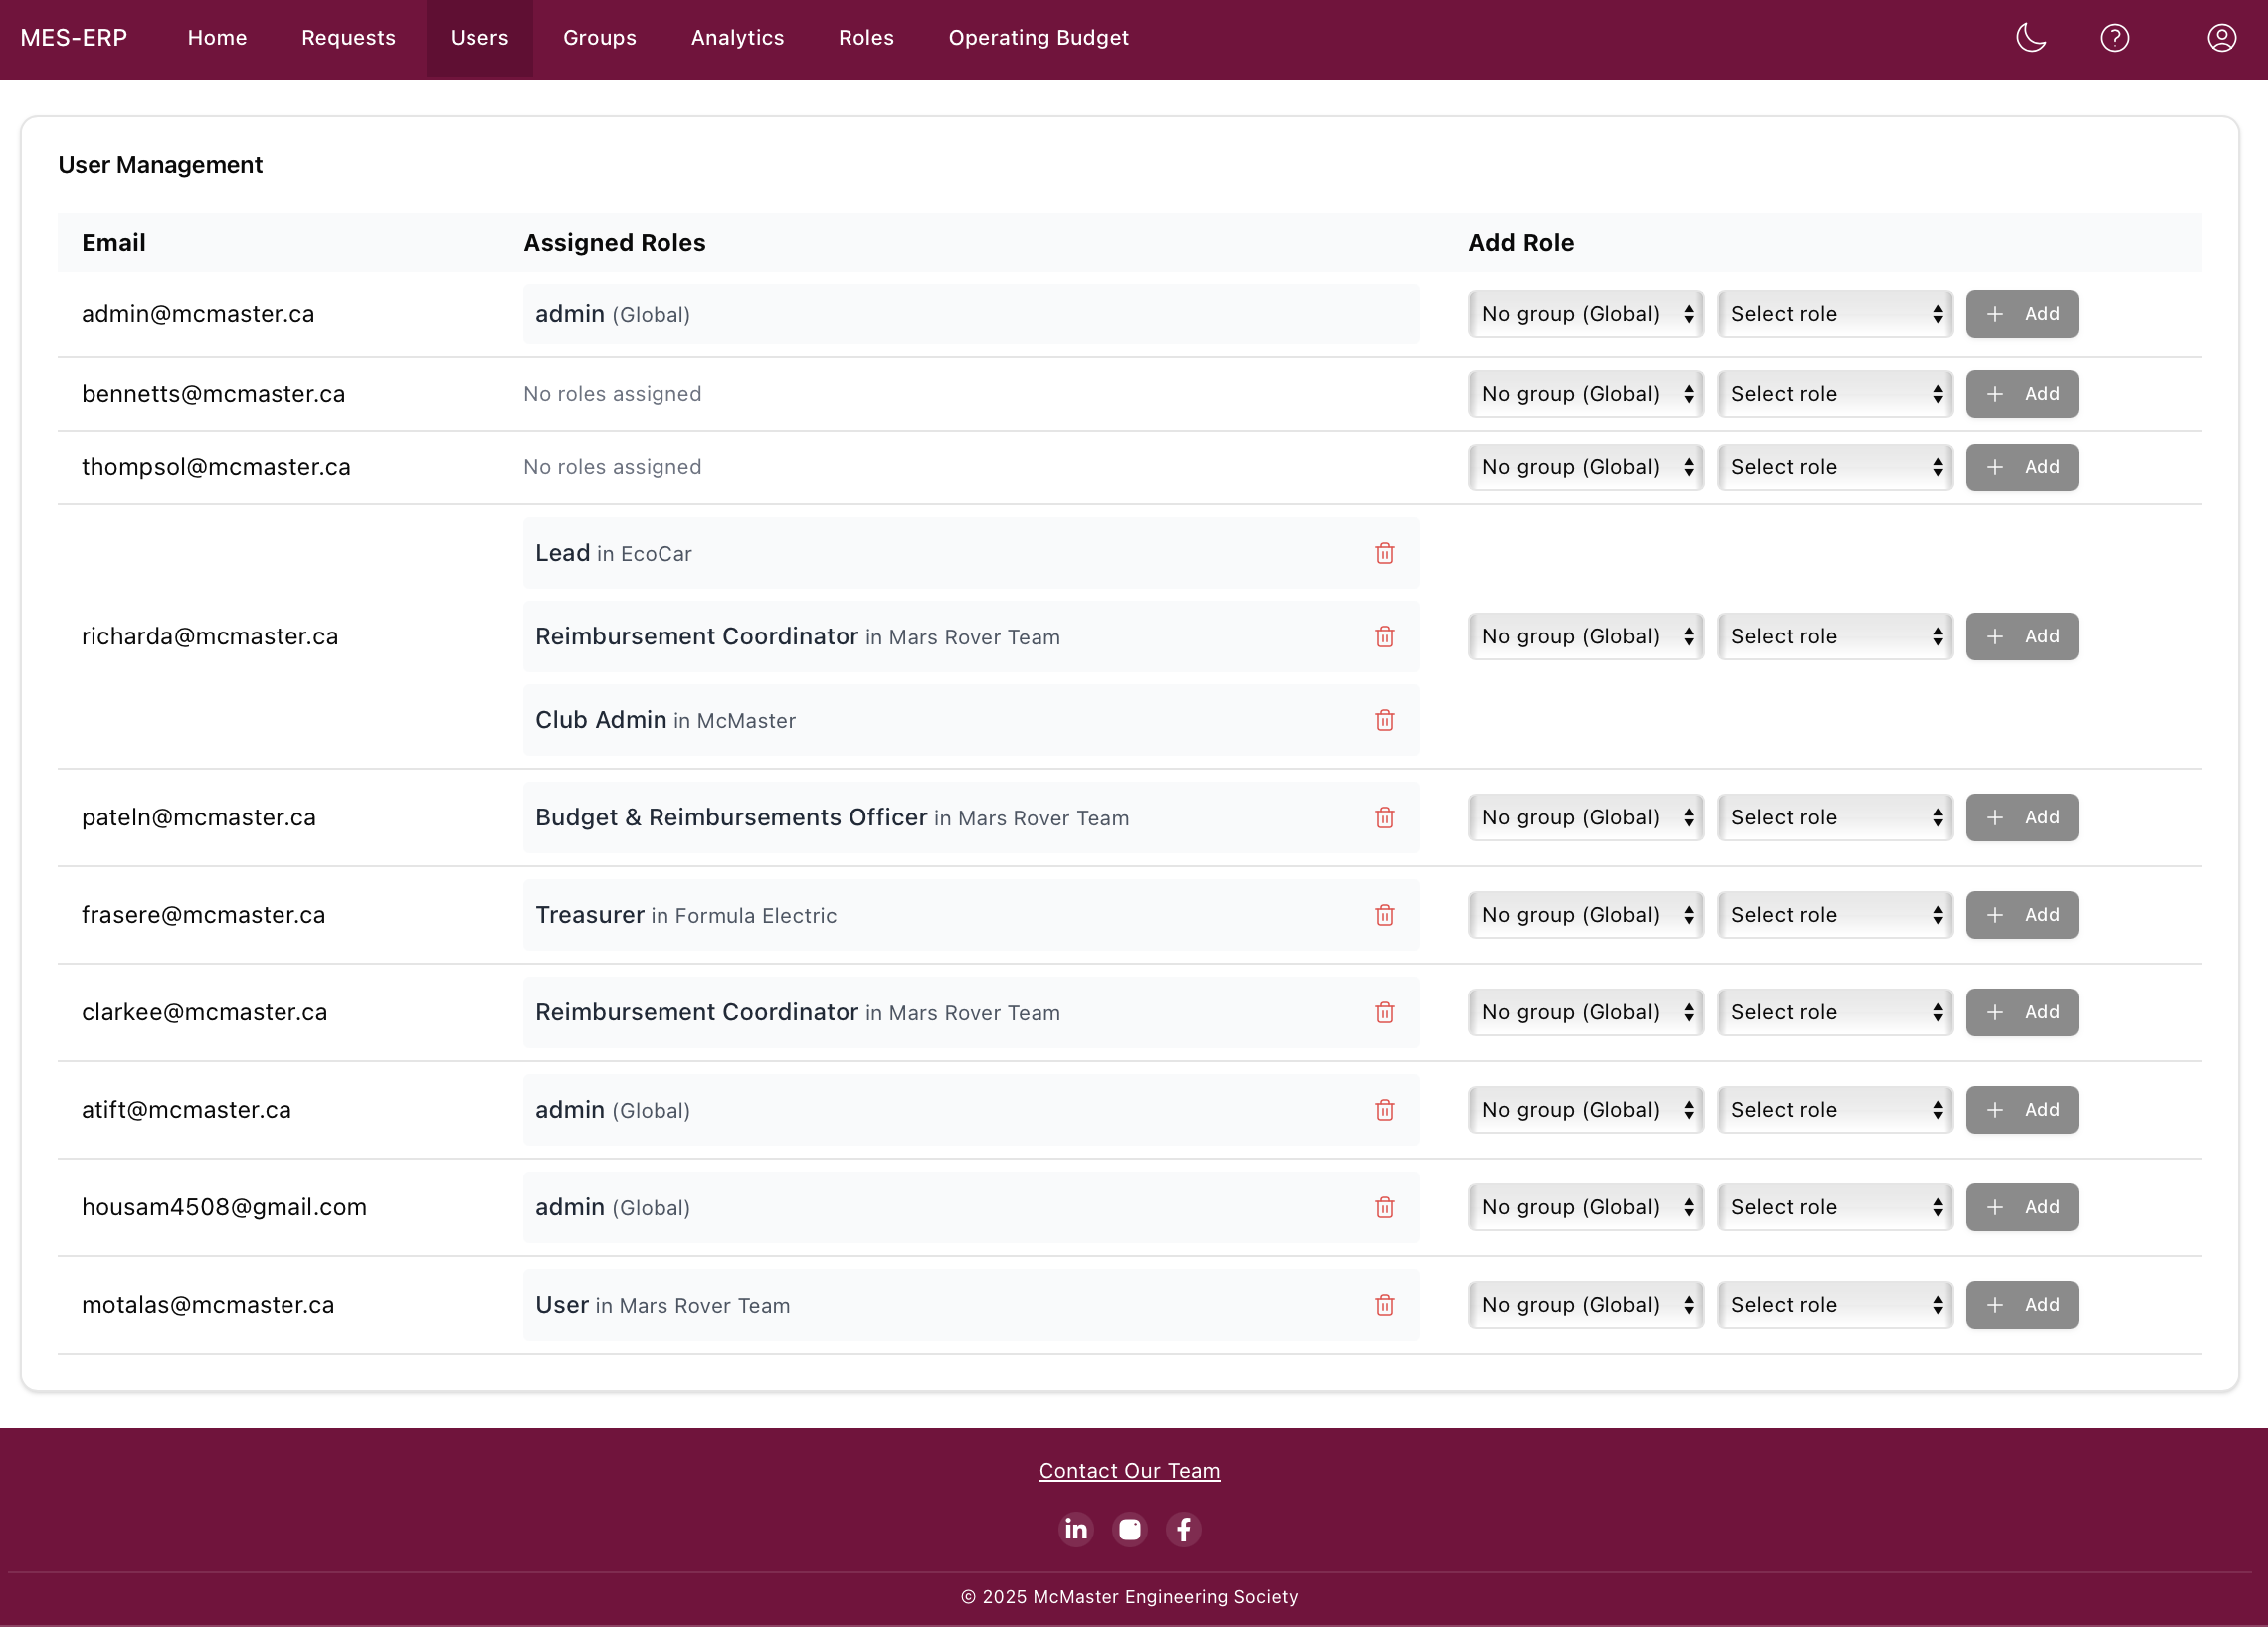
\includegraphics[width=0.8\textwidth]{users.png}
    \caption{Users Management Page}
\end{figure}

\clearpage
\subsection{(Optional) Managing Club Roles (\texttt{/dashboard/roles})}
(Requires \texttt{manage\_club\_roles} permission)
\begin{enumerate}
    \item Navigate to the \textbf{Roles} page.
    \item You can view, create, or modify roles \textit{that are specifically assigned to your group(s)}.
    \item You typically cannot create roles with high-level administrative permissions. Assign only the permissions needed for club operations.
\end{enumerate}

\begin{figure}[H]
    \centering
    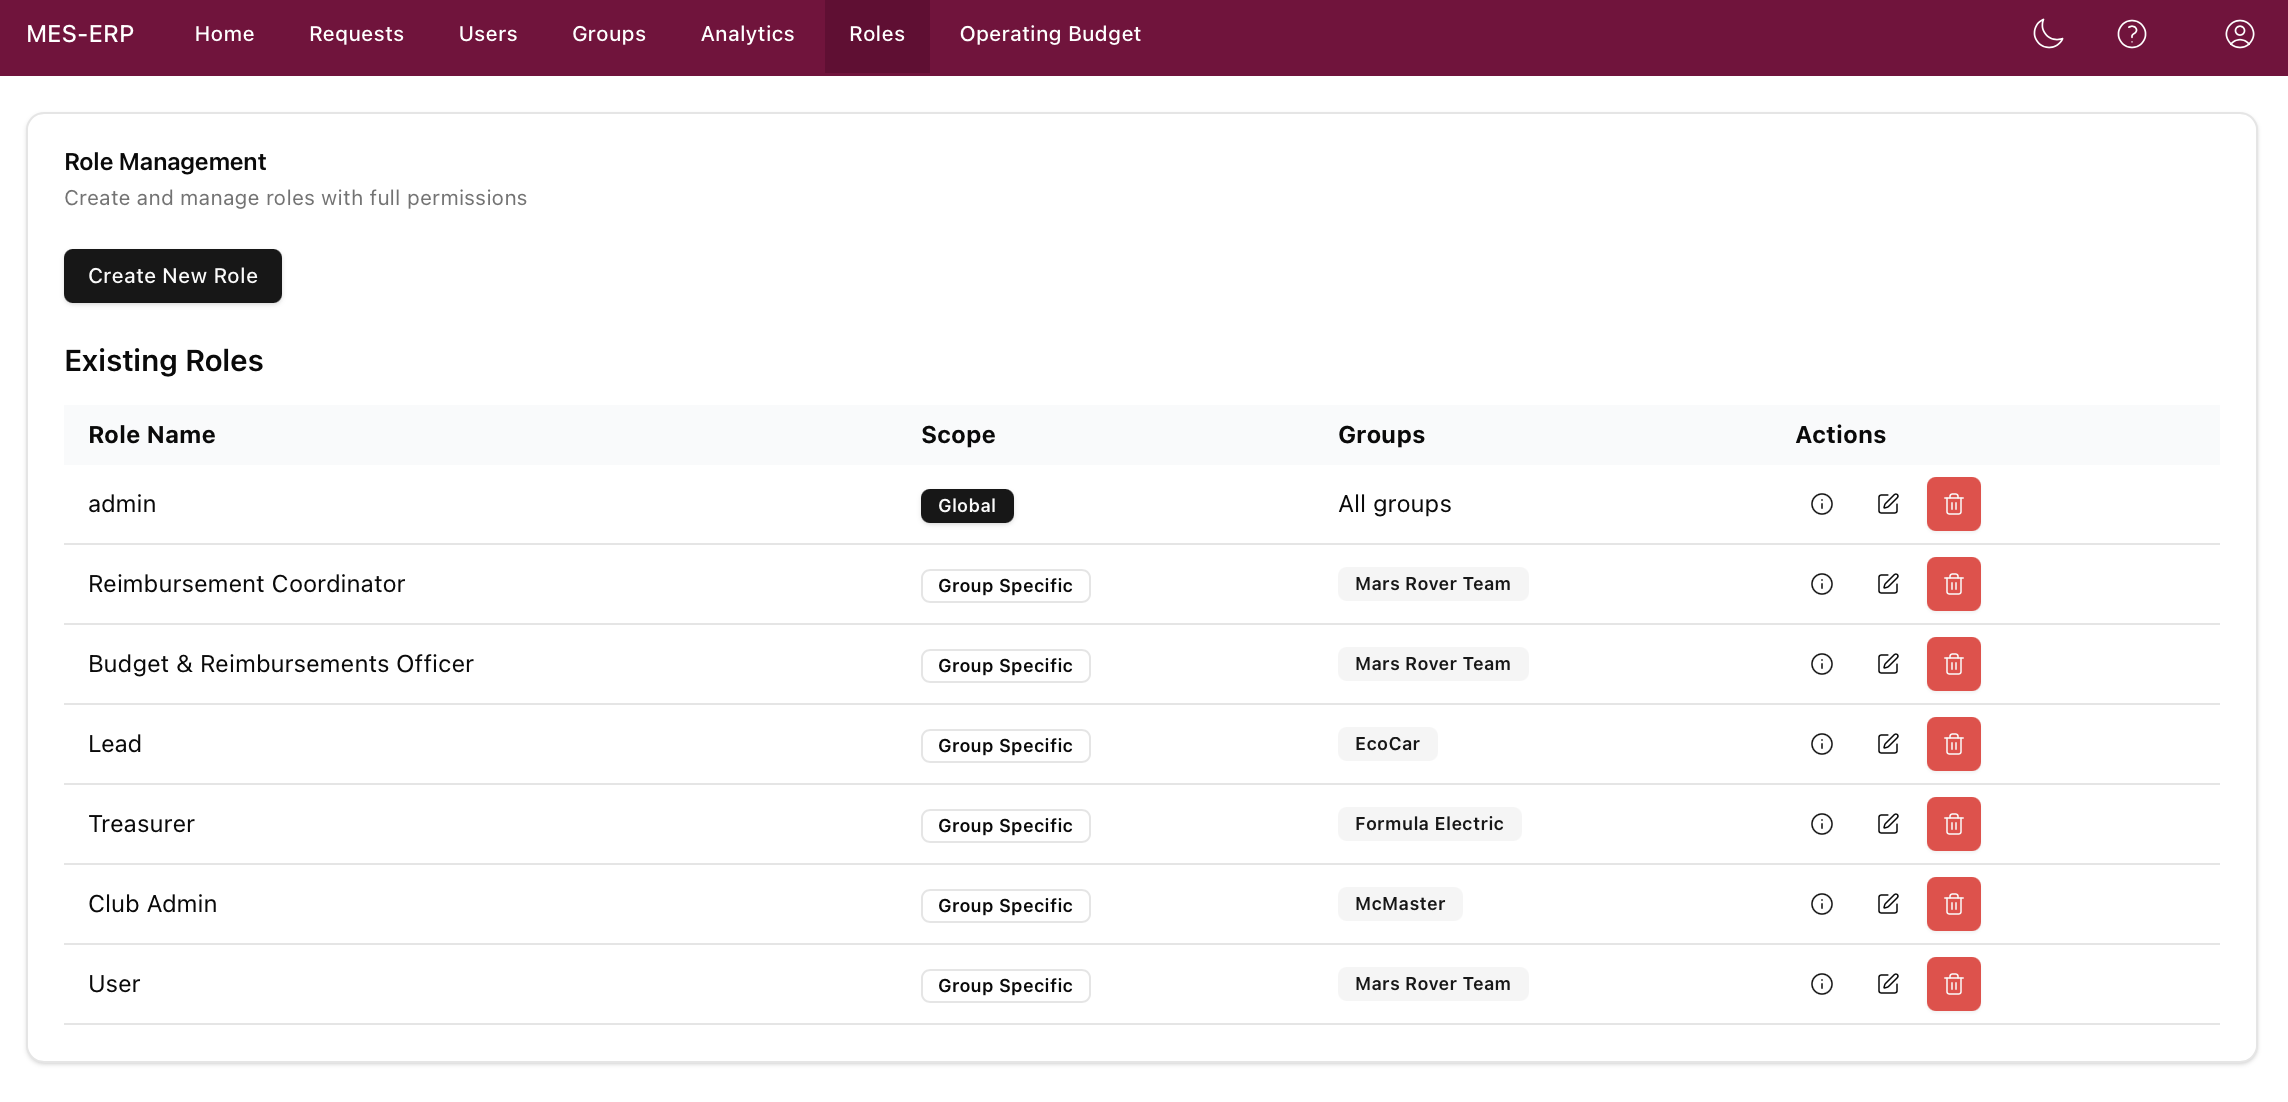
\includegraphics[width=0.8\textwidth]{roles.png}
    \caption{Roles Management Page}
\end{figure}

\subsection{Managing Groups (\texttt{/dashboard/groups})}
\begin{enumerate}
    \item Navigate to the \textbf{Groups} page.
    \item Click \textbf{Create New Group} to add a new club/organization.
    \item Edit group names directly in the table (if enabled) or via an edit action.
    \item Delete groups using the Delete (trash) icon (typically only if no users or roles are assigned to them).
\end{enumerate}

\begin{figure}[H]
    \centering
    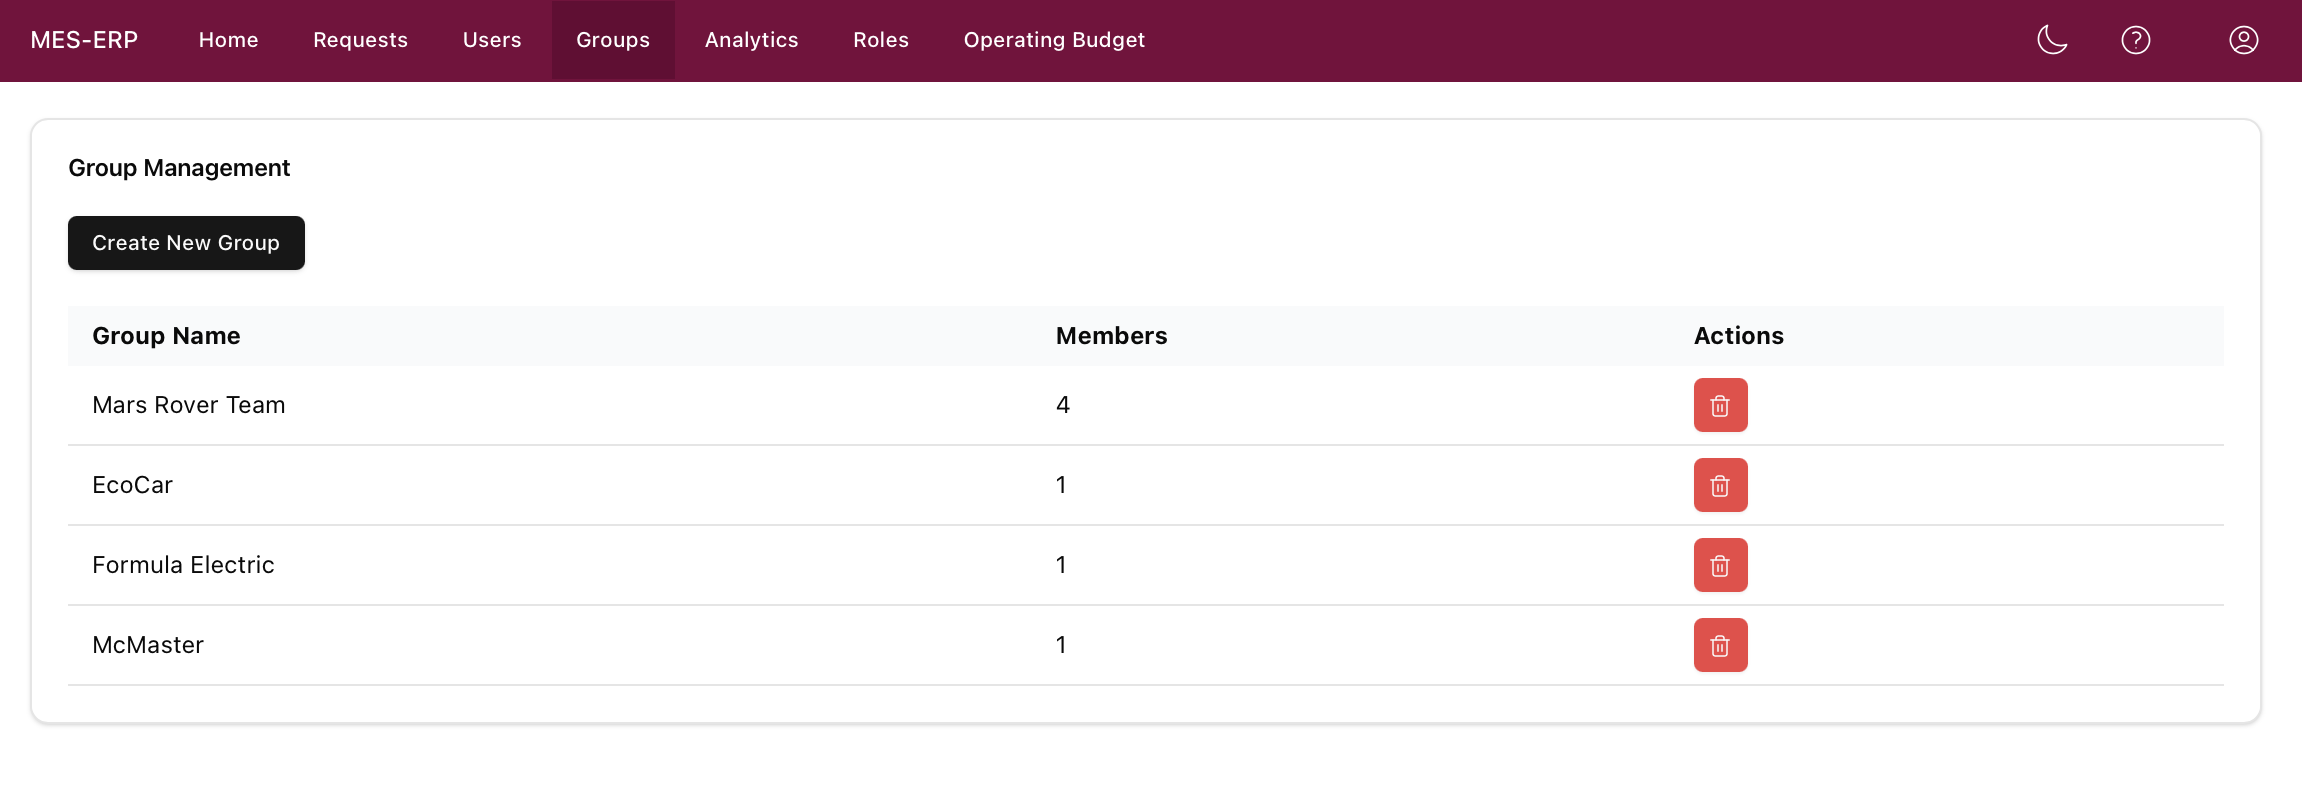
\includegraphics[width=0.8\textwidth]{groups.png}
    \caption{Groups Management Page}
\end{figure}

\clearpage
\subsection{Managing the Operating Budget (\texttt{/dashboard/operating\_budget})}
\begin{enumerate}
    \item Navigate to the \textbf{Operating Budget} page.
    \item This interface allows detailed management of group budgets.
    \item Add/remove groups using the buttons.
    \item Add/remove budget line items within groups using the "+ Add Row" and "Remove" buttons.
    \item Edit allocated amounts for different budget years (e.g., \texttt{col\_2024\_2025}) and line item labels directly in the table cells. The Change column (\texttt{col\_change}) is usually calculated automatically.
    \item Reorder rows within a group by dragging and dropping.
    \item Use the \textbf{Save All} button to persist changes made on the page.
\end{enumerate}

\begin{figure}[H]
    \centering
    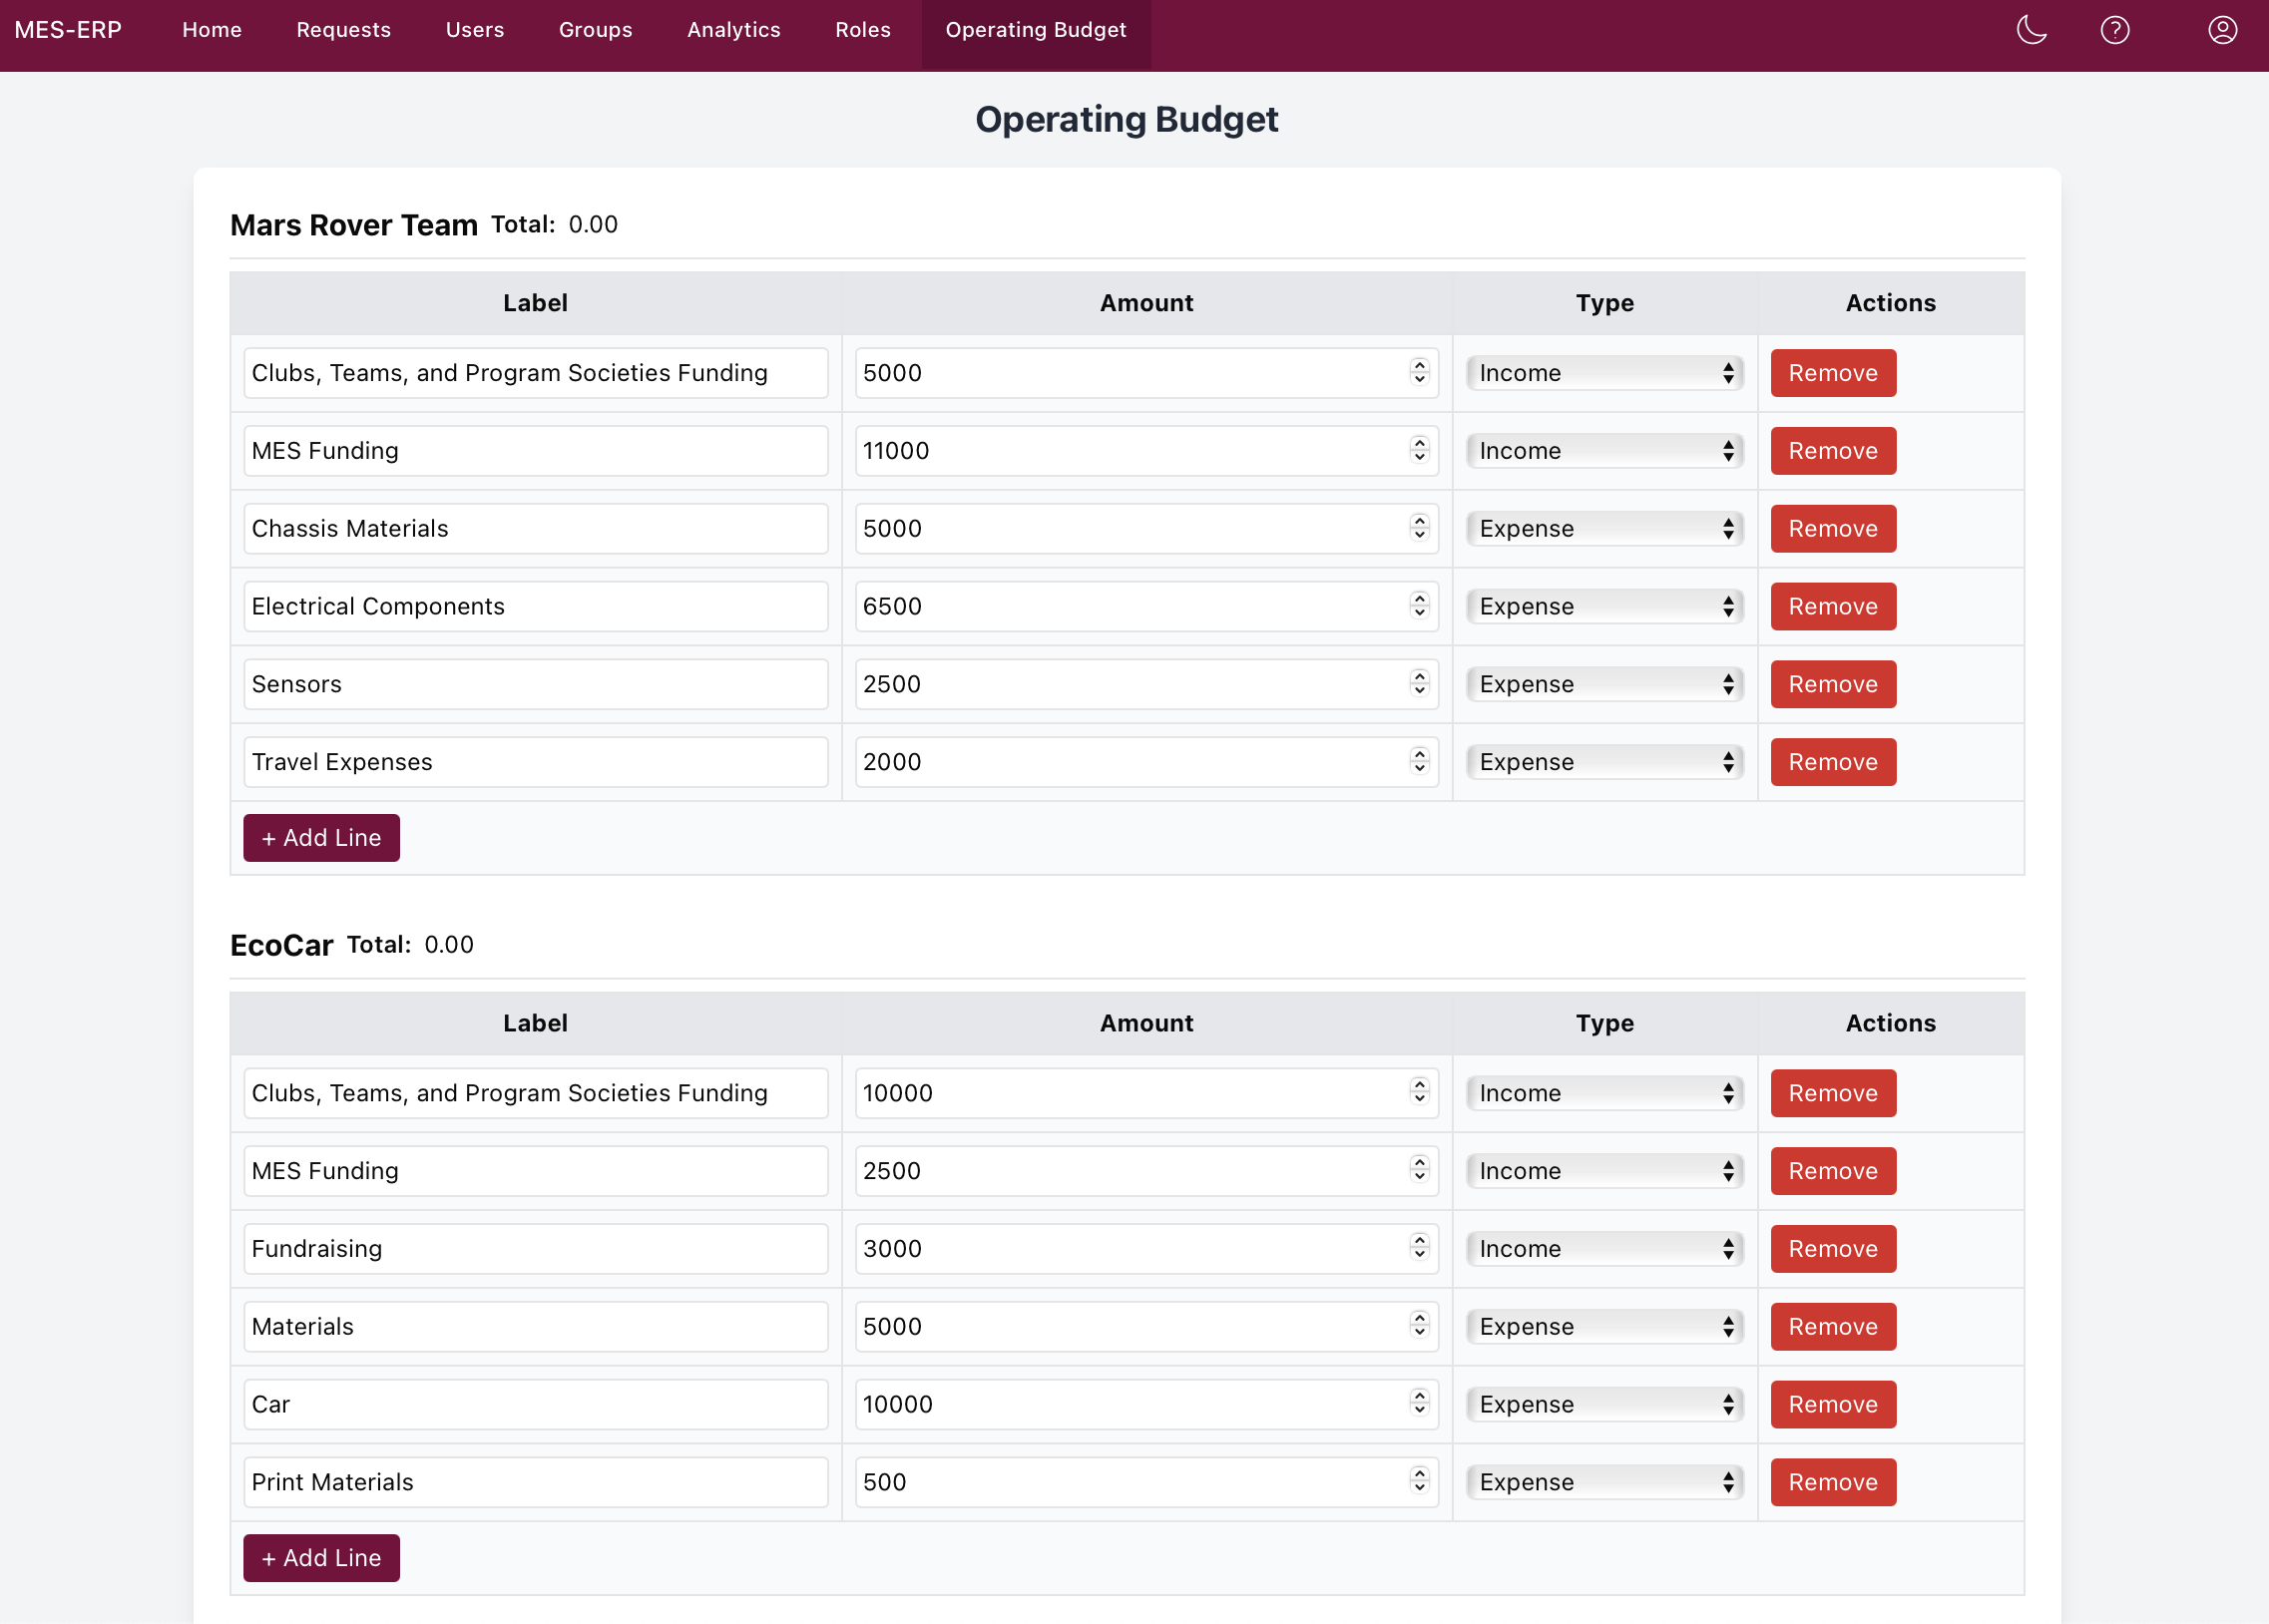
\includegraphics[width=0.8\textwidth]{operating_budget.png}
    \caption{Operating Budget Page}
\end{figure}

\subsection{Viewing System Analytics (\texttt{/dashboard/analytics})}
\begin{enumerate}
    \item Navigate to the \textbf{Analytics} page.
    \item View dashboards and charts summarizing financial activity across the \textit{entire system}.
    \item Analyze spending trends, status distributions, group spending, budget utilization, etc. Use the tabs ("Overview", "Detailed Analysis") for different views.
\end{enumerate}

\begin{figure}[H]
    \centering
    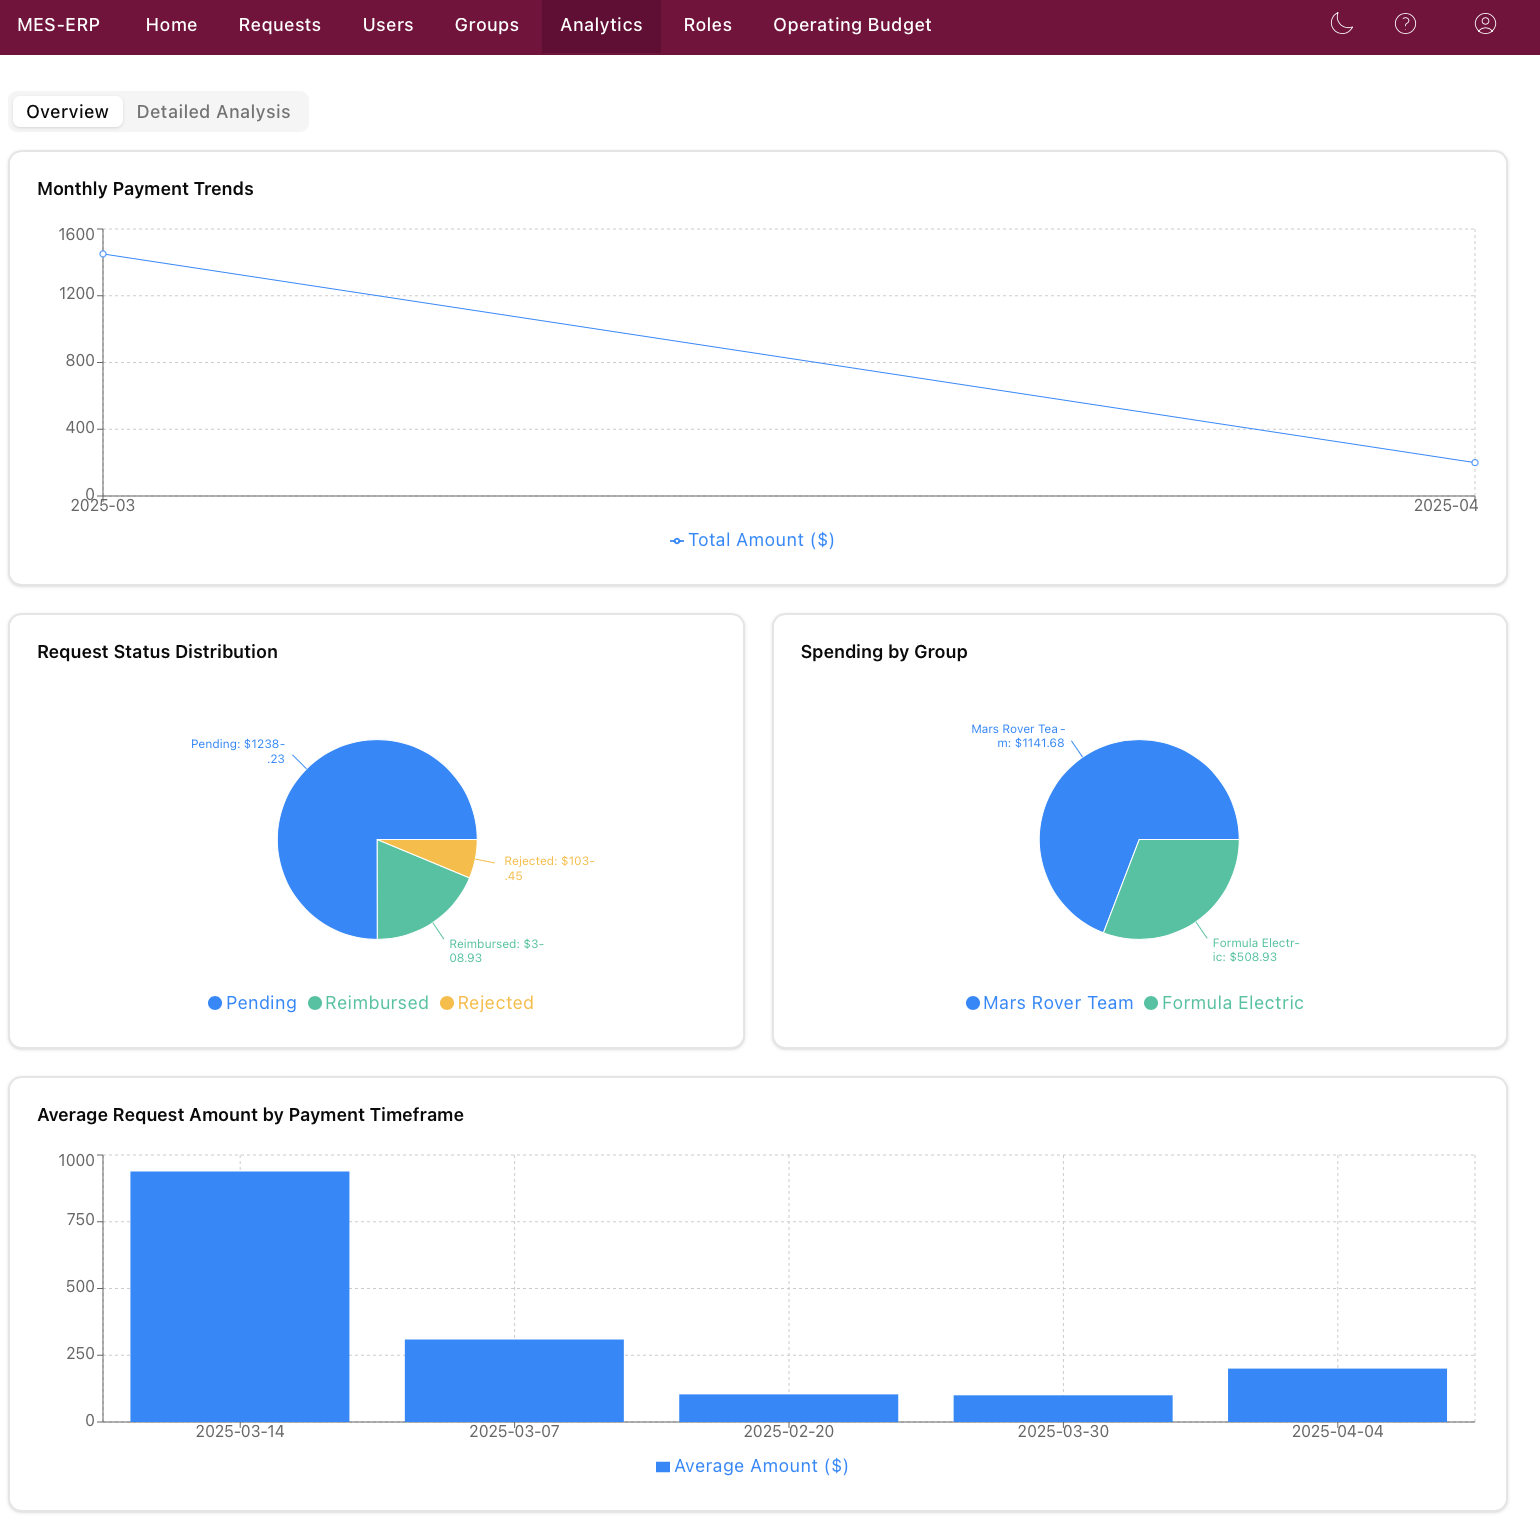
\includegraphics[width=0.8\textwidth]{analytics.png}
    \caption{Analytics Page}
\end{figure}

\clearpage
\section{Key Features Overview}

\begin{itemize}
    \item \textbf{Reimbursement Form \& OCR:} The \texttt{/forms} page allows detailed submission of requests. It includes an OCR feature to automatically read the total amount from uploaded receipt images (PDF, JPG, PNG).
    \item \textbf{Budget Management:} The \texttt{/dashboard/operating\_budget} page provides a powerful interface for admins to manage detailed budget lines for all groups. The \texttt{/dashboard/annual\_form} allows clubs to submit their yearly budget requests.
    \item \textbf{Role-Based Access Control (RBAC):} The system uses a flexible RBAC model where permissions are tied to roles, and roles can be global or specific to certain groups. Users can hold multiple roles across different groups.
    \item \textbf{Notifications (Email/SMS):} Users are automatically notified via email (and potentially SMS if phone numbers are configured and Twilio is set up) when the status of their payment requests changes.
    \item \textbf{Analytics Dashboard:} The \texttt{/dashboard/analytics} page offers various charts and tables to visualize financial data, helping with oversight and decision-making.
\end{itemize}

\section{Troubleshooting \& FAQ}

\begin{itemize}
    \item \textbf{I can't log in.}
        \begin{itemize}
            \item Ensure you are using the correct email and password.
            \item Try resetting your password via the link on the login page (if available).
            \item If you registered recently, check your email for a confirmation link.
            \item Contact MES support if problems persist.
        \end{itemize}
    \item \textbf{Why can't I see requests from other clubs?}
        \begin{itemize}
            \item Access is based on your assigned roles and permissions. Regular users typically only see their own requests. Club Admins see requests for their specific club(s). Only System Admins can see all requests.
        \end{itemize}
    \item \textbf{My request status hasn't changed.}
        \begin{itemize}
            \item Processing times can vary. Please allow a few business days for review. You will receive a notification when the status is updated. If it takes unusually long, contact your club admin or MES Finance.
        \end{itemize}
    \item \textbf{The OCR didn't read my receipt amount correctly.}
        \begin{itemize}
            \item OCR accuracy can depend on image quality and layout. Please manually verify and correct the "Amount Requested" field in the form if the OCR result is inaccurate.
        \end{itemize}
\end{itemize}

\section{Contact Information}

For technical issues or questions about using the \progname{} platform, please contact:
\begin{itemize}
    \item MES ERP Support: \textit{[motalas@mcmaster.ca]}
    \item MES Finance: \textit{[schuurml@mcmaster.ca]}
\end{itemize}

% --- End of User Guide Content ---

\end{document}